\documentclass{esannV2}
\usepackage{graphicx}
\usepackage[latin1]{inputenc}
\usepackage{amssymb,amsmath,array}
\usepackage{parskip}
\usepackage{multicol}

\voffset 0 cm \hoffset 0 cm \addtolength{\textwidth}{0cm}
\addtolength{\textheight}{0cm}\addtolength{\leftmargin}{0cm}


\begin{document}
%style file for ESANN manuscripts
\title{DNA als opslagmedium}

\author{Stijn Rosaer$^1$ - Olivier Van Houtte$^2$
\vspace{.3cm}\\
1- Universiteit Antwerpen - Computer Science \\
Prinsstraat 13 2000 Antwerpen - Belgium
}
\maketitle

\begin{abstract}
Zoals we weten, is er interesse in het opslaan van data als DNA. Er bestaan al veel methoden om dit DNA op te bouwen en terug uit te lezen, maar de encoderings wijze staat nog niet vast. In dit verslag achterhalen we of er misschien tijd en/of plaats effici\"entere encoderings systemen zijn dan gewoon bit voor bit op te slaan en of deze in de praktijk toepasbaar zijn. 
\end{abstract}

\section{Inleiding}
Als we aan DNA denken, worden we al snel herinnerd aan de 4 basen. Adenine (A), Guanine (G), Cytosine (C) en Thymine (T). Met deze basen kunnen we de eenvoudigste vorm van encoding opstellen, namenlijk 2 bits per base. We kiezen dan voor elke base een unieke combinatie aan bits.
\newline

00 = A, 01 = G, 10 = C, 11 = T
\newline


We kunnen dan elke DNA string (met een even aantal bits) omzetten naar DNA.
\newline

0111001110 $\rightarrow$ GTATC
\newline

Het kan echter effici\"enter. 


\section{Encodering}

In plaats van simpelweg 2 bits aan elke base toe te wijzen, stellen we nu eerst alle mogenlijke sets op, bestaande uit unieke combinaties van de 4 basen. Er zijn er zo 15.

\begin{center}
\begin{multicols}{3}
	
\begin{enumerate}
\item A
\item G
\item C
\item T
\item A G
\item A C
\item A T
\item G C
\item G T
\item C T
\item A G C
\item A G T
\item A C T
\item G C T
\item A G C T
\end{enumerate}

\end{multicols}
\end{center}

We kunnen de combinaties bestaande uit meerdere basen linken aan \textit{degenerate bases} volgens de standaard.

\begin{center}
\begin{tabular}{ c | c }
	A & A \\
	G & G \\
	C & C \\
	T & T \\
	R & A G\\
	M & C T\\
	Y & A C\\
	K & G T\\
	S & C G\\
	W & A T\\
	H & A C T\\
	B & C G T\\
	V & A C G\\
	D & A G T\\
	N & A C G T\\
\end{tabular}
\end{center}

Wanneer we deze voorstelling zouden bekijken voor DNA strings opgebouwd uit de hierboven gedefinieerde \textit{degenerate bases} kunnen we in een plot zien hoe deze verspreid worden en dus eenvoudig te identificeren zijn.

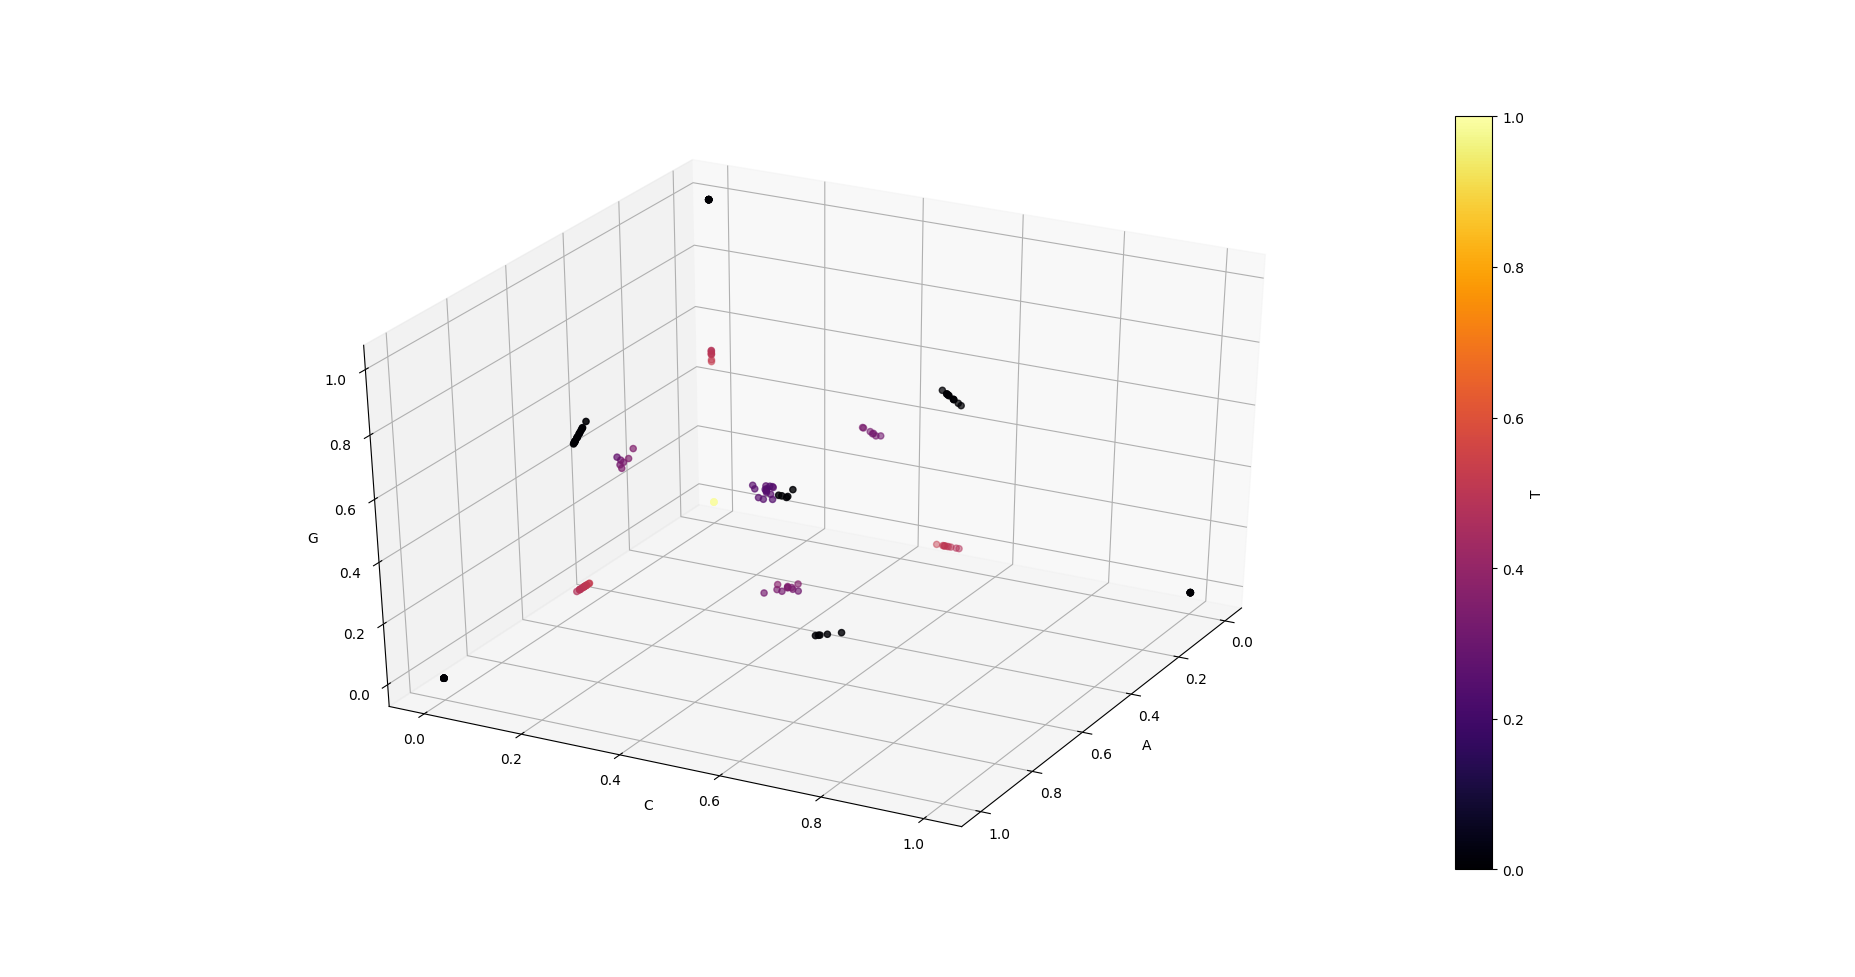
\includegraphics[scale=0.35]{img/theoretical.png}
\newpage

Door gebruik te maken van deze 15 combinaties zouden we theoretisch $\log_{2}{15}$ of 3.9 bits kunnen encoderen per base.
We kunnen aan deze combinaties hier de getallen 0 t.e.m. 14 toewijzen. We zouden dus, om alles correct te kunnen voorstellen 4 bits nodig hebben, wat meer is dan het theroetisch maximum. Hierdoor moeten we 1 bit minder gebruiken voor de encoding en komen dus op een mogelijke encoding van 3 bits per base.
Met deze 3 bits kunnen we de getallen 0 t.e.m. 7 voorstellen. Hierdoor kiezen we 8 sets ($2^{3}$ in plaats van alle 15 combinaties.
We geven ze ook telkens een nieuwe letter wanneer de sets meer dan 1 base bevatten, zodat we deze makkelijker in string vorm kunnen representeren. Hiervoor maken we gebruik van de IUPAC standaard voor \textit{degenerate base symbols}.

   
\begin{center}
\begin{tabular}{ c || c | c c |c}
	A & 0 & A && 000\\
	G & 1 & G && 001\\
	C & 2 & C && 010\\
	T & 3 & T && 011\\
	R & 4 & A & G& 100\\
	M & 5 & C & T& 101\\
	Y & 6 & A & C& 110\\
	K & 7 & G & T& 111\\
\end{tabular}
\end{center}

We kunnen nu weer een string van bits omzetten naar een string, gerepresenteerd door de gekozen sets. Indien het aantal bits niet deelbaar is door 3, voegen we de nodige nullen toe aan het begin van de string waardoor elke base de representatie is van exact 3 bits.

$$(00)0111001110 \rightarrow AKGY$$

Om de nodige DNA strings te verkrijgen, kiezen we voor elke letter een base uit de corresponderende set.
Waneer we een reeks data willen encoderen door DNA zullen we in dit geval, voor elke 3 bits, een corresponderende \textit{degenerate base} vinden in de hierboven gedefini\"eerde tabel. Aangezien sommige bases een combinatie zijn van Adenine, Cytosine, Guanine en Thymine, zullen we meerdere DNA strings moeten genereren ter encodering van een base op positie i in het resultaat om de overeenkomstige positie in elke string terug te vinden.
\newline
\begin{center}
\begin{tabular}{c}
	A K GCA Y \\
	\hline
	A$|$G$|$GCA$|$A$|$\\
	A$|$C$|$GCA$|$T$|$\\
	A$|$G$|$GCA$|$T$|$\\
	A$|$C$|$GCA$|$A$|$\\
	...\\
\end{tabular}
\end{center}
\newpage

We bouwen nu zoveel strings als nodig is, wat zeer effici\"ent kan met moderne technieken.
Wanneer we de data terug willen decoden, kiezen we weer een aantal DNA strings uit de gegenereerde strings.
We controleren welke basen we terug vinden, en achterhalen zo welke corresponderende letter hier mee overeen komt.
\newline

Wanneer we alle gegenereerde data in een plot plaatsen, kunnen we zien welke verdeling we hier hanteren.

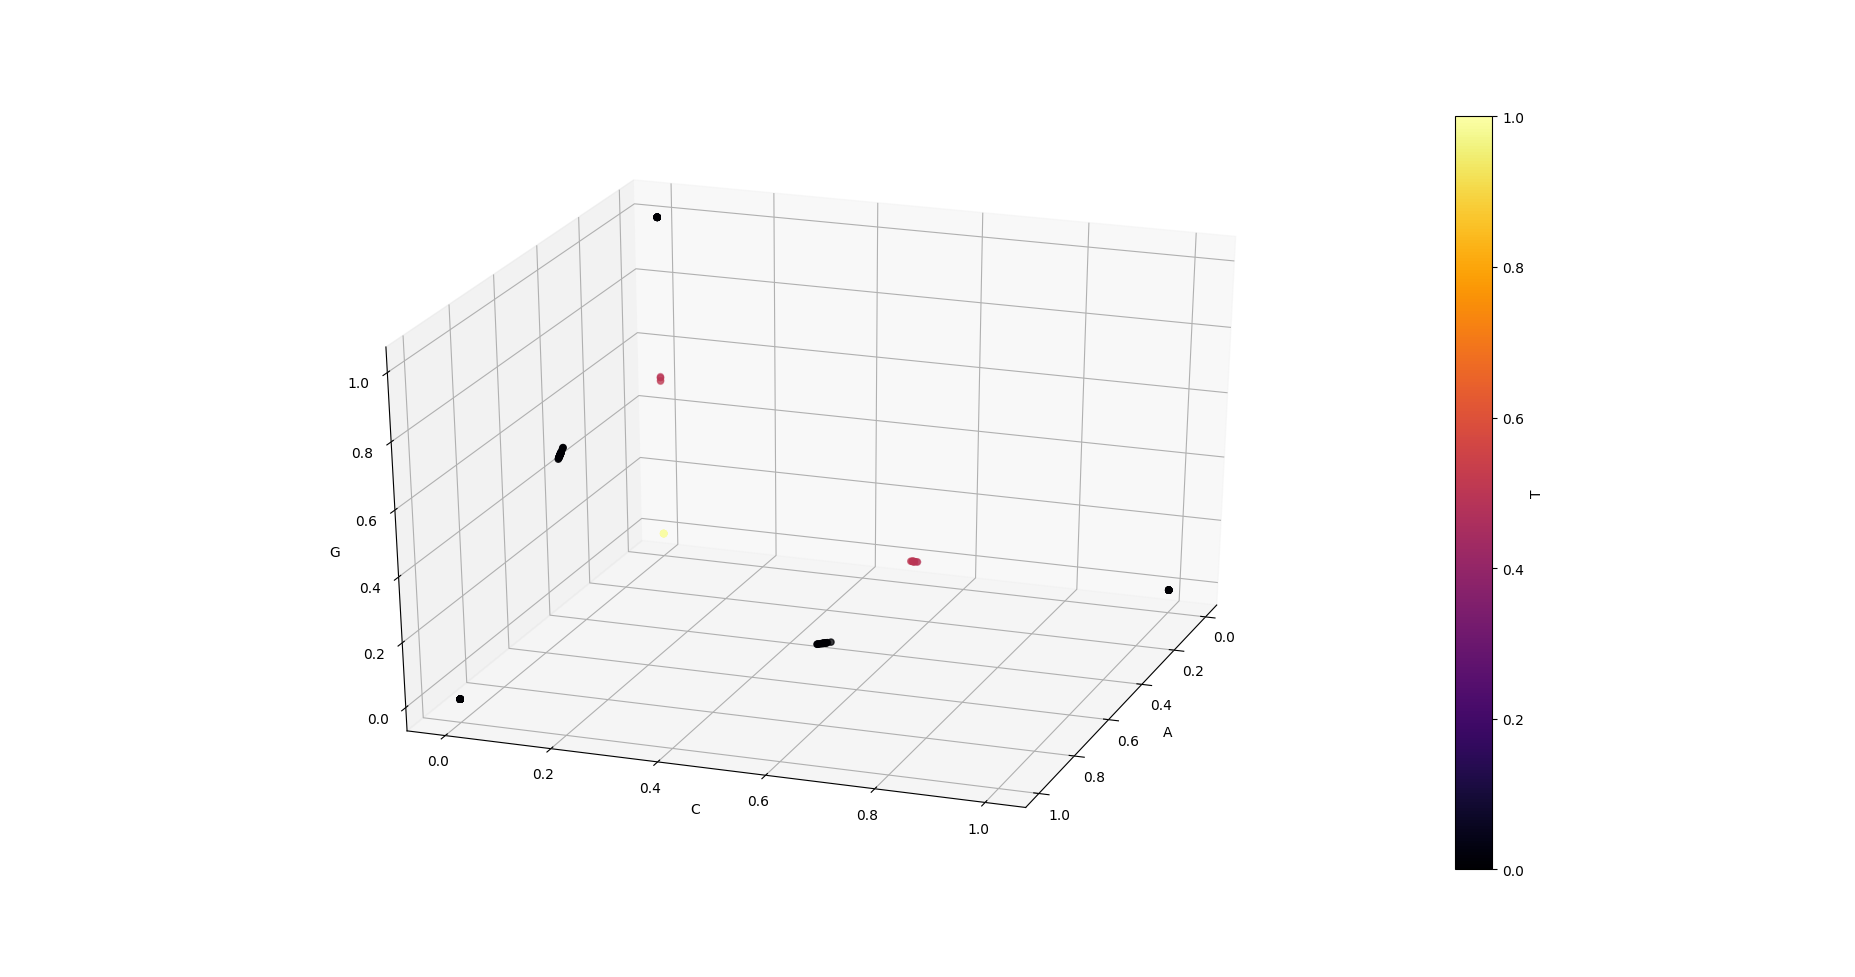
\includegraphics[scale=0.35]{img/practical.png}

\subsection*{Voorbeeld}
 We zien op positie 3, in verschillende strings, de characters A en C. Dan weten we dat dit een Y representeert.

Stel dat er maar 1 soort base wordt gelezen op een bepaalde positie. Dan zijn er meerdere opties. 

\begin{itemize}
	\item We lezen inderdaad een letter met maar 1 base in zijn set. Correct.
	\item We lezen een letter met 2 basen in zijn set, maar zien maar 1 base in onze gekozen strings. Fout. 
\end{itemize}

Dit zorgt ervoor dat we niet altijd de correcte output terugkrijgen. 

\newpage
\section{Correctheid}
De kans op het correct lezen van een character:

$$1-\left(\frac{1}{2}\right)^{N}$$

\newline
Dat maakt de kans op een volledig correct gelezen string:

$$\left(1-\left(\frac{1}{2}\right)^{N}\right)^L$$

Met L het aantal characters in de DNA strings en N het aantal strings dat we gebruiken om te controleren.

Onze tests komen zeer goed overeen met deze formule. 
We testen hier met een input DNA string van lengte L = 144. Vervolgens trachten we voor een toenemend aantal random gekozen DNA strings uit een set van 1000 proberen de originele data te recupereren. Dit herhaalden we voor elk aantal 500 keer en bekwamen onderstaand resultaat.
\newline

\begin{center}
\begin{tabular}{c|| c | c || c}
	N & tests ($\%$) & formule ($\%$) & verschil \\
	\hline
	4 & 0.0 & 0.0 & 0.0\\
	5 & 1.5 & 1.0  & 0.5\\
	6 & 12.3 & 10.4 & 1.9\\
	7 & 35.6 & 32.3 & 3.3\\
	8 & 58.6 & 57.0 & 1.6\\
	9 & 77.6 & 75.3 & 2.3\\
	10 & 88.3 & 86.9 & 1.4\\
	11 & 93.3 & 93.2 & 0.1\\
	12 & 97.2 & 96.5 & 0.7\\
	13 & 98.6 & 98.2 & 0.4\\
	14 & 99.3 & 99.1 & 0.2\\
	15 & 99.7 & 99.6 & 0.1\\
	16 & 99.8 & 99.8 & 0.0\\
	17 & 99.9 & 99.9  & 0.0\\
	18 & 99.9 & 99.9  & 0.0\\
	19 & 100 & 100  & 0.0\\
	...  & ... & ... & ...\\
	
	$\infty$ & 100 & 100  & 0.0\\
	
\end{tabular}
\end{center}

We verklaren de kleine verschillen door afrondings fouten.


\section{In de praktijk}

Het is eevoudiger om meerdere korte DNA strings te maken en lezen dan 1 lange. Dat is exact wat we met deze vorm van encoding doen. We maken i.p.v. 1 lange DNA string, veel korte, die we dan ook parallel kunnen inlezen indien nodig.
\newline

Zoals we weten bestaat DNA uit 2 strings. Opdat we zeker de juiste kant kiezen tijden het omzetten, kunnen we best elke DNA string beginnen en eindigen met een primer sequentie. Een kort stukje DNA van een vaste vorm, die het begin/ einde en de ori\"entatie van het DNA aanduidt. Dit verlengt onze DNA string een beetje, maar zou een relatief kleine impact hebben op het eindresultaat.
\newline

Indien we grotere hoeveelheden data willen opslagen, is het niet meer mogelijk om dit te doen in 1 enkele DNA string. Dit kunnen we oplossen door naast gebruik te maken van de primer ook een aantal basen toe te voegen die een index representeren van waar de DNA string in het resultaat moet komen. Dit geeft de mogelijkheid om alle DNA meer parallel uit te lezen. Grotere strengs zouden ook als probleem geven dat de kans op fouten bij het uitlezen groter wordt. De stijging in succes rate is echter zeer snel.\\
Stel dat we 1 terrabyte willen opslaan, komen we met het lezen van 50 strings al op een  succes rate van 99,8 $\%$. Dit is als we er vanuit gaan dat alles op 1 string gezet kan worden. Grote strings is dus een probleem dat, in de toekomst, met betere apparatuur opgelost kan worden.

\newpage
\section{Uitbreidingen}

We hebben tot nu toe steeds gewerkt met de 4 standaard basen. In theorie is er echter de mogenlijkheid om artifici\"ele basen toe te voegen. We zien hier 2 mogenlijkheden. 

\subsubsection*{Synthetische Basen}
Er is al onderzoek gedaan naar synthetische basen. Een voorbeeld hiervan zijn de Hachimoji basen. Deze verdubbelen het aantal mogenlijke basen die we in onze DNA strings kunnen gebruiken. Met meer basen, komen meer \textit{degenerated bases}, en dus meer bits per base. Een nadeel van de Hachimoji basen is dat ze niet in de natuur voorkomen en ze een constante aanvoer van bouwstenen en proteinen nodig hebben. Ze kunnen dus buiten een gecontroleerde omgeving niet gemaakt of onderhouden kunnen worden.

\subsubsection*{RNA}
RNA lijkt zeer sterk op DNA. Het gebruikt Uracil in plaats van Thymine en is enkelstrengig. Beide deze verschillen zouden nuttig kunnen zijn bij het opslaan van data. Een enkele streng halveert het biologisch materiaal nodig. Een nadeel is wel de levensduur van RNA. Wanneer we dus voor een langere periode gegevens willen opslagen is RNA niet geschikt als drager. We verliezen ook de capaciteit van de replicatie van DNA


\section{Conclusie}

We hebben nu reeds een methode gevonden om 3 bits te encoderen per DNA base door gebruik te maken van degenerate bases. Ook zijn we er van overtuigd dat er nog betere uitbereidingen zijn, zoals synthetische basen om docker tegen het theoretisch maximum te geraken. Indien de methoden voor het synthetiseren van DNA strings verbeterd, zal het lezen van, door op onze manier ge\"encodeerde gegevens, nog sneller kunnen verlopen. Indien er mutaties zouden optreden in het DNA moeten we er voor zorgen dat door gebruik te maken van correctie methoden deze errors opgelost worden.

Er is dus zeker nog meer onderzoek mogenlijk naar DNA als data storage. Onze inspiratie voor deze paper was dan ook een artikel uitgebracht vorig jaar$^1$. Maar wij vinden dit al zeker een zeer goede encoding.


\newpage
\begin{footnotesize}

\begin{thebibliography}{99}
	\bibitem{webArtikel} Choi, Y., Ryu, T., Lee, A.C. et al. High information capacity DNA-based data storage with augmented encoding characters using degenerate bases. Sci Rep 9, 6582 (2019). https://doi.org/10.1038/s41598-019-43105-w

	\bibitem{webArtikel hachimoji}S. Hoshika, N. A. Leal, M.-J. Kim, M.-S. Kim, N. B. Karalkar, H.-J. Kim, A. M. Bates, N. E. Watkins, H. A. SantaLucia, A. J. Meyer, et al., Science 2019, 363, 884–887
    https://science.sciencemag.org/content/363/6429/884
    
    \bibitem{webArtikel iupac}
    Stothard P (2000) The Sequence Manipulation Suite: JavaScript programs for analyzing and formatting protein and DNA sequences. Biotechniques 28:1102-1104.
    https://www.bioinformatics.org/sms2/iupac.html
    

\end{thebibliography}
\end{footnotesize}

\section*{Appendix A}
Bijhorende python bestanden zijn te vinden op github in de repository\\ https://github.com/OlivierVanHoutte/BioProject.

Door main.py uit te voeren met python3 kan de output verkregen worden. Onderaan bij de variable 'input' kan een andere string gedefinie\"erd worden.

\end{document}